\documentclass[12pt,a4paper,titlepage]{article}
\usepackage[utf8]{inputenc}
\usepackage[naustrian]{babel}
\usepackage[T1]{fontenc}
\usepackage{geometry}
\usepackage{fancyhdr}

%theorem
\usepackage{amsthm}
\theoremstyle{definition}
\newtheorem*{definition*}{Lösungsansatz}
\newtheorem{definition}{Lösungsansatz}
\newtheorem*{remark*}{Wichtig}


%graphic
\usepackage{graphicx}
\graphicspath{{images}}

% layout
\geometry{left=20mm, right=20mm, top=35mm, bottom=40mm}
\pagestyle{fancy}
\title{Design Patterns}
\author{Lukas Wais}
\setlength{\parindent}{0em} 

%sourcecode
\usepackage{listings}
\usepackage{color}
 
\definecolor{codegreen}{rgb}{0,0.6,0}
\definecolor{codegray}{rgb}{0.5,0.5,0.5}
\definecolor{codepurple}{rgb}{0.58,0,0.82}
\definecolor{backcolour}{rgb}{0.95,0.95,0.92}
 
\lstdefinestyle{mystyle}{
    backgroundcolor=\color{white},   
    commentstyle=\color{codegreen},
    keywordstyle=\color{blue},
    numberstyle=\tiny\color{codegray},
    stringstyle=\color{codepurple},
    basicstyle=\footnotesize,
    breakatwhitespace=false,         
    breaklines=true,                 
    captionpos=b,                    
    keepspaces=true,                 
    numbers=left,                    
    numbersep=5pt,                  
    showspaces=false,                
    showstringspaces=false,
    showtabs=false,                  
    tabsize=2,
    frame=single
}
 
\lstset{style=mystyle}

% footer
\fancyfoot{} 
%\fancyfoot[R]{Lukas Wais (11816105){\tiny }}
%\fancyfoot[L]{\LaTeX-Übung 2, erstellt: \today}
\fancyfoot[C]{\thepage}

\begin{document}
\maketitle

%Decorator
\section{Dekorator}
Dieses Muster soll es erlauben, zur Laufzeit eine zusätzliche Funktionalität zu einem vorhandenen Objekt in dynamischer Weise hinzuzufügen.
\subsection{Definition}
\begin{definition*}
In einem Dekorierer soll das zu verzierende, sprich das zu erweiternde Objekt zu aggregieren (verbinden) und gleichzeitig einem Kunden, dem Client, dieselbe Schnittstelle wie die zu verzierende Komponente angeboten werden.
\end{definition*}

Soll der Dekorierer eine bestimmte Methode der zu dekorierenden Klasse um eine zusätzliche Funktionalität erweitern so überschreibt er diese Methode. Um die bestehende Funktion zu nutzen, ruft der Dekorierer in der überschreibenden Methode die überschriebene Methode des aggregierten Objekts auf.

 \begin{remark*}
 Ein Dekorierer muss alle geerbten Methoden überschreiben.
 \end{remark*}

\subsection{UML - Diagramme}

\begin{figure}[htbp]
\begin{center}
\includegraphics[width=0.5\textwidth]{/decorator.png}

\caption{UML-Diagramm Dekorierer}
\label{default}
\end{center}
\end{figure}

\begin{figure}[htbp]
\begin{center}
\includegraphics[width=0.5\textwidth]{/decoratorMult.png}

\caption{UML-Diagramm mehrere Dekorierer}
\label{default}
\end{center}
\end{figure}

\newpage

\subsection{Konkretes Beispiel}

\begin{figure}[htbp]
\begin{center}
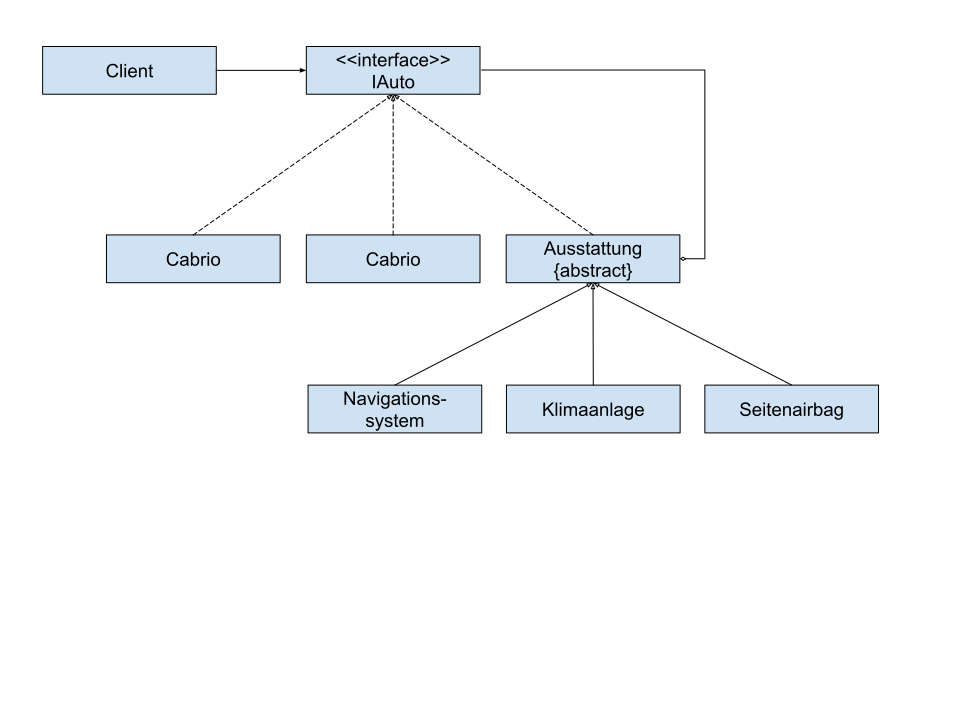
\includegraphics[width=1\textwidth]{/UMLAuto}

\caption{UML-Diagramm Dekorierer}
\label{default}
\end{center}
\end{figure}

\begin{lstlisting}[language=Java, caption=IAuto.java]
public interface IAuto {

	public int gibKosten();
	public void zeigeDetails();
}
\end{lstlisting}

\newpage

\begin{lstlisting}[language=Java, caption=Cabrio.java]
class Cabrio implements IAuto {
	public void zeigeDetails() {
		System.out.print("Cabrio");
	}

	public int gibKosten() {
		return 50000;
	}
}
\end{lstlisting}

\begin{lstlisting}[language=Java, caption=Ausstattung.java]
public abstract class Ausstattung implements IAuto {
	protected IAuto auto;

	public Ausstattung(IAuto pIAuto) {
		auto = pIAuto;
	}
}
\end{lstlisting}

\begin{lstlisting}[language=Java, caption=Klimaanlage.java]
class Klimaanlage extends Ausstattung {
	public Klimaanlage(IAuto pIAuto) {
		super(pIAuto);
	}

	// "dekoriert" die Details
	public void zeigeDetails() {
		auto.zeigeDetails();
		System.out.print(", Klimaanlage");
	}

	// "dekoriert" die Kosten
	public int gibKosten() {
		return auto.gibKosten() + 1500;
	}
}
\end{lstlisting}

\newpage

\begin{lstlisting}[language=Java, caption=Navigationssystem.java]
class Navigationssystem extends Ausstattung {
	public Navigationssystem(IAuto pIAuto) {
		super(pIAuto);
	}

	// "dekoriert" die Details
	public void zeigeDetails() {
		auto.zeigeDetails();
		System.out.print(", Navigationssystem");
	}

	// "dekoriert" die Kosten
	public int gibKosten() {
		return auto.gibKosten() + 2500;
	}
}
\end{lstlisting}

\begin{lstlisting}[language=Java, caption=Seitenairbag.java]
class Seitenairbags extends Ausstattung {
	public Seitenairbags(IAuto pIAuto) {
		super(pIAuto);
	}

	// "dekoriert" die Details
	public void zeigeDetails() {
		auto.zeigeDetails();
		System.out.print(", Seitenairbags");
	}

	// "dekoriert" die Kosten
	public int gibKosten() {
		return auto.gibKosten() + 1000;
	}
}
\end{lstlisting}

\newpage

\begin{lstlisting}[language=Java, caption=Client.java]
class Client {
	
	// Auto mit Klimaanlage
	public static void main(String[] args) { 
		IAuto auto = new Klimaanlage(new Limousine());
		auto.zeigeDetails();
		System.out.println("\nfuer " + auto.gibKosten() + " Euro\n");

		// Dynamische Erweiterung der Limousine mit Ausstattungen
		auto = new Navigationssystem(new Seitenairbags(auto));
		auto.zeigeDetails();
		System.out.println("\nfuer " + auto.gibKosten() + " Euro\n");

		// Cabrio Variante
		auto = new Navigationssystem(new Seitenairbags(new Cabrio()));
		auto.zeigeDetails();

		System.out.println("\nfuer " + auto.gibKosten() + " Euro\n");
	}
}
\end{lstlisting}

\subsection{Vor- und Nachteile}
\subsubsection{Vorteile}
\begin{itemize}
	\item Flexibler als Vererbung.
	\item Weniger Klassen nötig.
	\item Funktionalität beliebig (tief) zusammensetzbar.
	\item Funktionalität zur Laufzeit änderbar (hinzufügbar und entfernbar).
	\item Dekorierte Klasse bleibt erweiterbar.
\end{itemize}

\subsubsection{Nachteile}
\begin{itemize}
\item Etwas ineffizienter (durch Forwarding).
\item Dekorator $\neq$ dekoriertes Objekt (keine Objektidentität).
\item Auch Zugriffe zu Feldern müssen über Methoden gehen.
\end{itemize}

%Visitor
\section{Besucher}
Das Besuchermuster soll es erlauben, die Daten aller Objekte einer Objektstruktur zentral auszuwerten.

\subsection{Definition}
\begin{definition*}
Ein wichtiges Kennzeichen des Besuchermusters ist es, dass die Objekte der Objektstruktur Instanzen von unterschiedlichen Klassen sein können.
\newline
Für jede zu realisierende Operation wird eine \textbf{Besucher-Klasse} bereitgestellt, die einen Satz von überladenen \textbf{visit()-Methoden} enthält und zwar jeweils eine separate visit()-Methode für jede in der Objektstruktur vorhandene Element-Klasse. 
\newline
Die \textbf{accept()-Methode} einer Element - Klasse hat als Übergabeparameter ein Besucher-Objekt . Das Objekt, dessen accept()-Methode aufgerufen wird, ruft im Rumpf der accept()-Methode die für eine Element - Klasse spezifische visit()-Methode des übergebenen Besuchers auf und \textbf{übergibt dabei eine Referenz auf sich selbst.}
\end{definition*}
\begin{lstlisting}[language=Java, caption=Beispiel Accept-Methode]
  @Override
  public <T> T accept(ExprVisitor<T> visitor) {
    return visitor.visit(this);
  }
\end{lstlisting}

\newpage

\subsection{Klassendiagramm}

\begin{figure}[htbp]
\begin{center}
\includegraphics[width=1\textwidth]{/visitor}

\caption{Klassendiagramm Visitor}
\label{default}
\end{center}
\end{figure}

\subsection{Konkretes Beispiel}

Die abstrakte Klasse MitarbeiterBesucher repräsentiert die abstrakte Besucher-Klasse und definiert für jede konkrete Element-Klasse, welche besucht werden soll.
\textbf{Visit-Methoden}
\lstinputlisting[language=Java, caption=Abstrakte Klasse MitarbeiterBesucher.java]{src/visitor/MitarbeiterBesucher.java}

\newpage

Die Klasse Gehaltsdrucker stellt einen konkreten Besucher dar und wird aus diesem Grund von der Klasse MitarbeiterBesucher abgeleitet. 
In den Implementierungen der jeweiligen visit()-Methoden werden \textbf{Informationen über das jeweils gerade besuchte Objekt ausgegeben.}
\lstinputlisting[language=Java, caption=Gehaltsdrucker.java abgeleitet von MitarbeiterBesucher]{src/visitor/Gehaltsdrucker.java}

Durch die Klasse Gesellschaft wird die Objektstruktur realisiert. Sie beinhaltet \\ \textbf{Beispielinstanzen der konkreten Objekte}.
\lstinputlisting[language=Java, caption=Gesellschaft.java]{src/visitor/Gesellschaft.java}

Die abstrakte Klasse Mitarbeiter ist die \textbf{Basisklasse für die konkreten Elemente} dieses Beispiels. Sie entspricht somit der abstrakten Klasse Element aus der allgemeinen Beschreibung des Besucher-Musters. 
Die abstrakte Klasse Mitarbeiter \textbf{gibt für konkrete Element-Klassen die Deklaration der abstrakten Methode accept() vor.}
\lstinputlisting[language=Java, caption=Abstrakte Klasse Mitarbeiter.java abgeleitet von MitarbeiterBesucher]{src/visitor/Mitarbeiter.java}

Die Klasse  Sachbearbeiter ist eine \textbf{konkrete Element-Klasse}. Sie ist von der abstrakten Klasse Mitarbeiter abgeleitet und implementiert die accept()-Methode.
\lstinputlisting[language=Java, caption=Klasse Sachbearbeiter.java abgeleitet von Mitarbeiter]{src/visitor/Sachbearbeiter.java}

\newpage

Die Klasse Teamleiter stellt ebenfalls eine \textbf{konkrete Element-Klasse} dar. Sie ist von der abstrakten Klasse Mitarbeiter abgeleitet und implementiert die von der abstrakten Klasse Mitarbeiter vorgegebene accept()-Methode.
\lstinputlisting[language=Java, caption=Klasse Teamleiter.java abgeleitet von Mitarbeiter]{src/visitor/Teamleiter.java}

\newpage

Innerhalb der main()-Methode der Klasse PersonalVerwaltung wird eine neue Objektstruktur als Objekt der Klasse Gesellschaft angelegt. Aus dieser kann die aktuelle Belegschaft in Form einer Mitarbeiterliste ermittelt werden. Die Belegschaft wird durchlaufen und die jeweiligen Mitarbeiter werden durch den Gehaltsdrucker \textbf{besucht}.
\lstinputlisting[language=Java, caption=Klasse PersonalVerwaltung.java mit der main()-Methode]{src/visitor/PersonalVerwaltung.java}

\newpage

\subsection{Vor- und Nachteile}
\subsubsection{Vorteile}
\begin{itemize}
	\item Einfaches Hinzufügen von neuer Funktionalität.
	\item Zentralisierung des Codes einer Operation.
	\item Möglichkeit Klassenhierarchien-übergreifender Besuche (nicht wie beim Iterator-Muster).
	\item Sammeln von Informationen.
	\item Verbesserung der Wartbarkeit.
	\item Möglichkeit Frameworks zu erweitern.
\end{itemize}

\subsubsection{Nachteile}
\begin{itemize}
	\item Hoher Aufwand beim Hinzufügen von Element-Klassen.
	\item Hoher Aufwand bei der nachträglichen Anwendung des Musters.
	\item Overhead (durch das simulierte Double Dispatch in der accept()-Methode entsteht zusätzlicher Aufwand, der die Performance verschlechtert).
	\item Aufweichung der Kapselung privater Daten.
\end{itemize}

\newpage

\section{Adapter}
Eine Klasse soll wiederverwendet werden. Die zu wiederzuverwendende Klasse bietet zwar die richtigen Daten an, hat aber eine unpassende Schnittstelle für den Zugriff eines Clients auf diese Daten.

\subsection{Definition}
\begin{definition*}
	Das Adapter-Muster hat zum Ziel, eine vorhandene \glqq falsche\grqq ~ Schnittstelle einer bereits vorhandenen Klasse an die vom Client gewünschte Form anzupassen.
\end{definition*}

\subsection{Klassendiagramm}
\subsubsection{Klassen-Adapter (Adapter mit Vererbung)}
Die Klasse Adapter verwendet für den Aufruf der \glqq alten\grqq ~Operationen einfach eine Selbstdelegation an den ererbeten Anteil.
Die zu adaptierende Klasse stellt die anzupassende Komponente dar.
\begin{figure}[htbp]
	\begin{center}
	\includegraphics[width=0.5\textwidth]{/kAdapter.png}
	
	\caption{Klassendiagramm Klassen-Adapter}
	\label{default}
	\end{center}
\end{figure}
\subsubsection{Objekt-Adapter (Adapter mit Delegation)}
Die Adapter-Klasse implementiert die Aufrufschnittstelle IZiel und delegiert den Aufruf an das 
aggregierte Objekt der zu adaptierenden Klasse weiter.
\begin{figure}[htbp]
	\begin{center}
	\includegraphics[width=0.5\textwidth]{/oAdapter.png}
	
	\caption{Klassendiagramm Objekt-Adapter}
	\label{default}
	\end{center}
\end{figure}

\subsection{Konkretes Beispiel}
Als Beispiel soll eine kleine Anwendung dienen, die Personendaten aus einer CSV-Datei ausliest.
Das Einlesen von CSV-Dateien aus einer Datei in einen Zwischenpuffer sei in diesem Beispiel schon von einer
Klasse implementiert worden, die vor längerer Zeit geschrieben wurde und deshalb \textbf{nicht} 
auf die Architektur der Anwendung, d.h. auf die Aufrufschnittstelle des Clients, abgestimmt ist.
Um diese Klasse zur Anwendung \textbf{kompatibel zu machen}, wird eine Adapter-Klasse eingesetzt.
\newline
\newline
Hierbei stellt die Klasse \textit{CSVLeser die zu adaptierende Klasse dar}, die Klasse \textit{CSVLeserAdapter den Adapter}
und die Klasse \textit{TestAdapter den Client}. Die Klasse CSVLeserAdapter muss das Interface IPersonenLeser implementieren.

\lstinputlisting[language=Java, caption=Person.java Hilfsklasse spielt keine Rolle im Adapter Muster]{src/adapter/Person.java}
\newpage

\lstinputlisting[language=Java, caption=CSVLeser.java die zu adaptierende Klasse]{src/adapter/CSVLeser.java}

\lstinputlisting[language=Java, caption=IPersonenLeser.java Schnittstelle für alle Klassen die Personendaten einlesen können]{src/adapter/IPersonenLeser.java}
\newpage

\lstinputlisting[language=Java, caption=CSVLeserAdapter.java Adapter für die Klasse CSVLeser]{src/adapter/CSVLeser.java}

\lstinputlisting[language=Java, caption=TestAdapter.java mit main()-Methode dient als Client]{src/adapter/TestAdapter.java}

\subsection{Vor- und Nachteile}
\subsubsection{Vorteile}
\begin{itemize}
	\item Ermöglicht Kommunikation zwischen zwei unabhängigen Softwarekomponenten.
	\item Adapter können um beliebig viele Funktionen erweitert werden (z.B. Filter).
	\item Sie sind individuell an die Lösung angepasst und können daher optimiert werden.
	\item Klassen können leicht ausgetauscht werden.
	\item Ein Adapter kann auch auf ein Objekt einer Unterklasse der zu adaptierenden Klasse angewandt werden.
\end{itemize}

\subsubsection{Nachteile}
\begin{itemize}
	\item Durch das Adapter-Muster wird beim Aufruf einer Operation ein zusätzlicher Zwischenschritt eingeführt, dies kann bei komplexen Adapter zu zeitlicher
	Verzögerung führen.
	\item Durch die individuelle Anpassung der Adapter auf die jeweilige Lösung weisen sie eine schlechte Wiederverwendbarkeit auf.
\end{itemize}

\newpage

%Komposite
\section{Composite}
Man möchte Teil-Ganzes-Hierachien erzeugen und dabei die Objekte in einer \textbf{baumartigen} Struktur gruppieren.
\newline

k \ldots Knoten
\newline
b \ldots Blatt

\begin{figure}[htbp]
	\begin{center}
	\includegraphics[]{/tree.png}
	
	\caption{Struktur einer Teil-Ganzes-Hierarchie}
	\label{default}
	\end{center}
\end{figure}

\begin{definition*}
Das Kompositum-Muster soll es erlauben, dass bei der Verarbeitung von Knoten in einer Baumstruktur einfache und zusammengesetzte Objekte gleich behandelt werden.
\newline
Durch den Einsatz des Kompositum-Musters wird es möglich, in einer Baumstruktur \textbf{zusammengesetzte Objekte} (Gruppen von Objekten) gleich wie einzelne \textbf{einfache} oder \textbf{primitive} Objekte, sogenannte Blätter zu behandeln. Dadurch wird der Aufwand im Client für die Verwaltung der resultierenden Baumstruktur verringert.
\end{definition*}

\subsection{Klassendiagramm}
\begin{figure}[htbp]
	\begin{center}
	\includegraphics[width=0.5\textwidth]{/kompositum.png}
	
	\caption{Struktur einer Teil-Ganzes-Hierarchie}
	\label{default}
	\end{center}
\end{figure}

\subsubsection{Teilnehmer}
\textbf{Konten} 
\newline
Die abstrakte Klasse \textit{Knoten} legt die Schnittstelle und das Verhalten der abgeleiteten Klassen \textit{Kompositum} und \textit{Blatt} fest. \\
Es wird ein \textbf{Defaultverhalten} für die Kindoperationen implementiert.
\newline

\textbf{Blatt}
\newline
Die Klasse \textit{Blatt} repräsentiert ein Knotenelement in der Baumstruktur, das \textbf{keine} weiteren Knoten aggregiert und selbst immer nur Kind-Knoten sein kann.
\newline

\textbf{Kompositum}
\newline
Die Klasse \textit{Kompositum} repräsentiert ein Knotenelement in der Baumstruktur, welches weiter Knoten aggregieren kann. Die Klasse \textit{Kompositum} implementiert die kindbezogenen Operationen und \textbf{überschreibt} damit das Defaultverhalten, das in der Klasse \textit{Knoten} implementiert ist.

\newpage

\subsection{Konkretes Beispiel}

\lstinputlisting[language=Java, caption=Knoten.java]{src/composite/Knoten.java}
Definiert die abstrakte Basisklasse Kompositum und Blatt werden davon abgeleitet.
\newpage

\lstinputlisting[language=Java, caption=Kompositum.java extends Knoten]{src/composite/Kompositum.java}
Überschreibt die kindbezogene Methoden und implementiert die ausgesuchte Operation operation().
\newpage

\lstinputlisting[language=Java, caption=Blatt.java extends Knoten]{src/composite/Blatt.java}
Repräsentiert eine einfche und nicht zusammengesetzte Knoten einer Baumstruktur und hat im Gegensatz zur Klasse Kompositum \textbf{keine} untergeordneten Knoten.

\subsection{Vor- und Nachteile}
\subsubsection{Vorteile}
\begin{itemize}
	\item Da ein Objekt der Klasse Blatt dieselbe Schnittstelle hat wie ein Objekt der Klasse Kompositum, kann der Client Blatt-Objekte und zusammengesetzte
	Kompositum-Objekte einheitlich behandeln. Dies vereinfacht die Handhabung der Baumstruktur durch den Client.
	\item Das Kompositum-Muster erlaubt es, verschachtelte Strukturen auf einfache Weise zu erzeugen bzw. um neue Blatt- und Kompositum-Klassen zu erweitern.
\end{itemize}

\subsubsection{Nachteile}
\begin{itemize}
	\item Das Design und der Aufbau der Baumstruktur werden unübersichtlich, wenn man viele unterschiedliche Blatt- und Kompositum-Klassen verwendet.
	\item Beim Kompositum-Muster werden alle Knoten gleich behandelt $\rightarrow$ nicht gut, wenn bei dem Aufbau einer Kompositum-Struktur gewissen
	Einschränkungen unterliegen soll. Diese Einschränkungen müssen durch Typüberprüfungen zur Laufzeit gewährleistet werden.
	\item Sobald Änderungen and der Basisschnittstelle vorgenommen werden, müssen potentielle alle davon abgeleiteten Klassen ebenfalls geändert werden.
\end{itemize}
\end{document}








